% Rules for the HuroCup Sprint Competition
% Jacky Baltes <jacky@cs.umanitoba.ca> 

\documentclass[12pt]{hurocup}

\newcommand{\thisyear}{2010}

\newcommand{\HuroCup}{\textsc{HuroCup}}


\begin{document}

\title{\HuroCup: Climbing Wall\\
  Laws of the Game \thisyear}

\author{Jacky Baltes\\
Autonomous Agents Laboratory\\
University of Manitoba\\
Winnipeg, Manitoba\\
Canada, R3T 2N2\\
Email: jacky@cs.umanitoba.ca\\
WWW: http://www.cs.umanitoba.ca/\~{ }jacky\\[5mm]
Kuo-Yang Tu\\
National Kaohsiung First University of Science and Technology\\
Kaohsiung City, R. O. C.\\
Email: tuky@ccms.nkfust.edu.tw\\
}

\maketitle

\begin{center}
 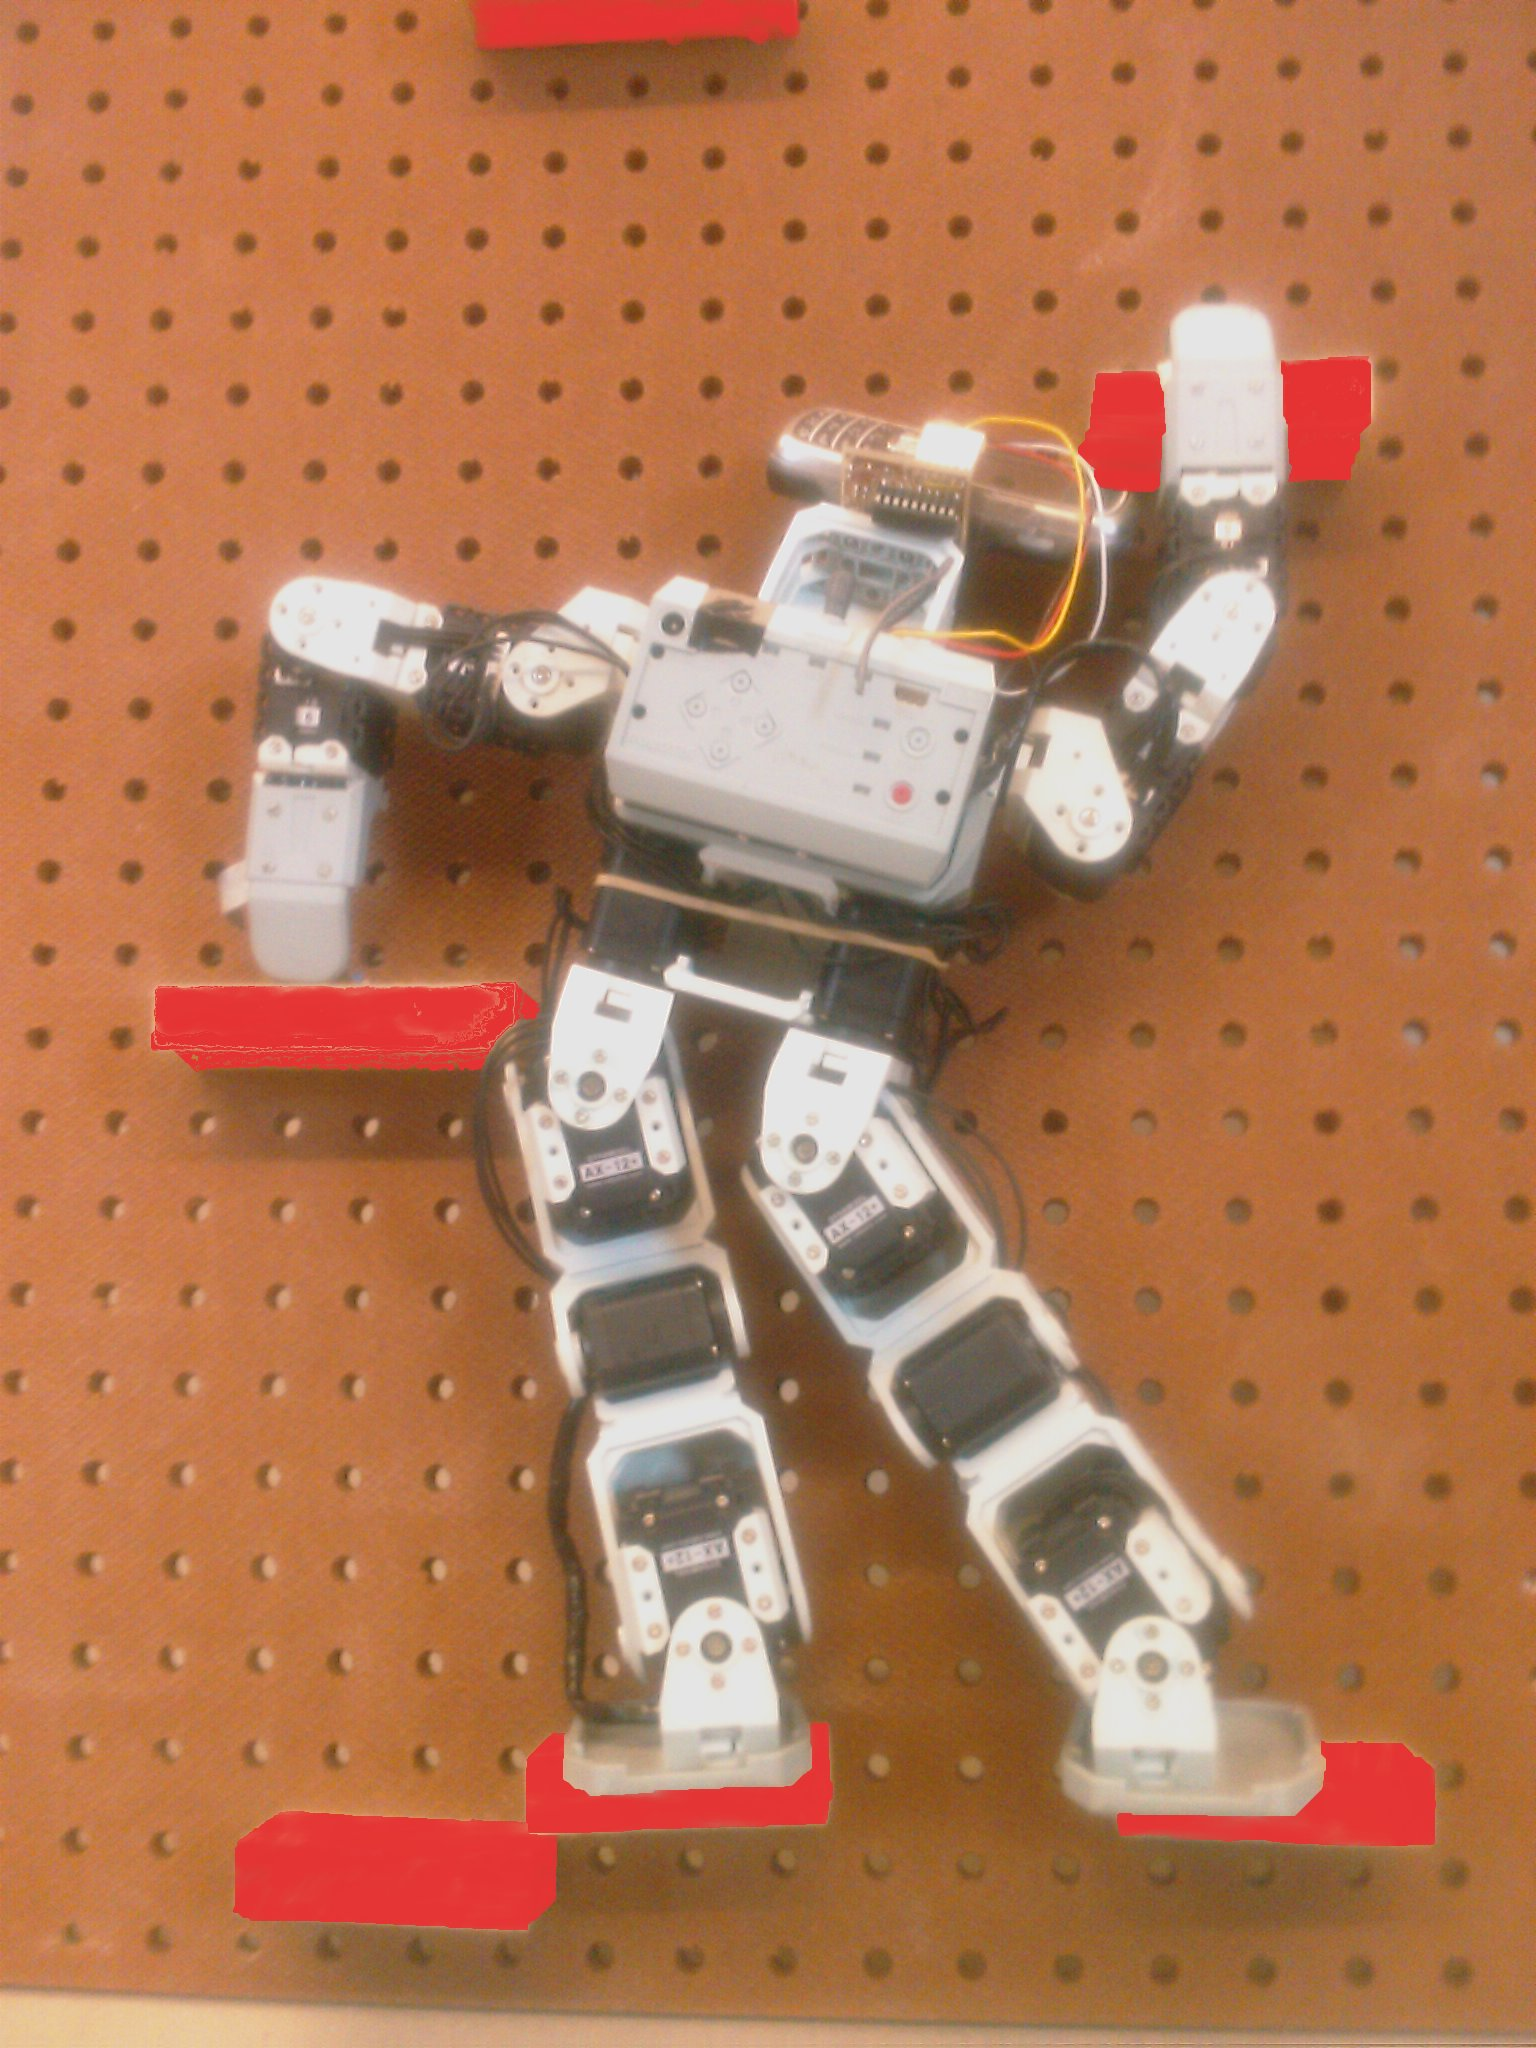
\includegraphics[width=0.4\linewidth]{Figures/climbing-wall}
\end{center}

\begin{abstract}
The following rules and regulations govern the game of the Climbing
Wall event in \HuroCup, a robotic game and robotics benchmark problem
for humanoid robots.
%
\end{abstract}

\section*{Latest Version of the Rules for \HuroCup}
\label{sec:updates}

The latest official version of the rules of the game for \HuroCup\ is
always available from the \HuroCup\ Facebook page
(http://www.facebook.com/groups/hurocup/).

\section*{Changes to the Rules of \HuroCup\ Climbing Wall for \thisyear}

No changes were made to the rules for \thisyear.

\newpage

\section{Climbing Wall}
\label{sec:climbing-wall}

The climbing wall challenge aims at fostering research into complex
motion plannng, coordination, and execution to increase the range of
usable motions for humanoid robots.

\section{Laws of the Game: Climbing Wall}
\label{sec:laws-climbing-wall}

The following laws describe the specifics of the climbing wall
event. For general specifications relevant to all \HuroCup\ events
(e.g., robot dimensions, playing field and lighting, responsibility of
the referees) please refer to the general \HuroCup\ laws.

\law[CW]{The Field of Play}
\label{law:field-of-play}

\begin{lawlist}[CW]

\item The dimensions of the playing field are at least 200 by
  200cm. 

\item At one end of the playing field, there is a climbing wall, which
  is at least 50cm wide and 100cm tall. 

\item The angle between the wall and the floor is between 75 degrees
  and 90 degrees.
  
\item The wall is built out of reinforced peg board or similar
  material. 

\item Several hand or foot holds are mounted on the wall. The size of
  the holds is either rectangular or circular. The size of the holds
  is at least 5cm by 5cm. The holds are strong enough to support a
  weight of at least 10kg. See Fig.~\ref{fig:climbing-wall-holds} for
  an example of rectangular and circular holds.\footnote{Thanks to
    Marco Wickrath for the Figure.}

\item The maximum distance between one hold and its nearest neighbor
  is at most 30cm.

\item Red markers are placed in the centre of the hand and foot holds
  to help a robot to detect the position of the holds using a vision
  system.

\end{lawlist}

\begin{figure}
  \begin{center}
    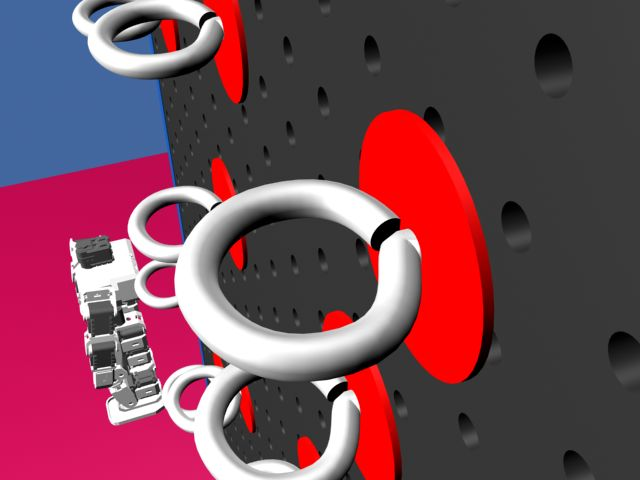
\includegraphics[width=0.45\linewidth]{Figures/climbing-wall2}
  \end{center}
  \caption{3D Rendering of Climbing Wall with Circular
    Holds}
  \label{fig:climbing-wall-holds}
\end{figure}

\law[CW]{Number of Robots}

\begin{lawlist}[CW]
\item A single robot competes in a match.
\end{lawlist}

\law[CW]{The Players}

Please refer to the general \HuroCup\ laws for a description of
the players.

\law[CW]{The Referee}

Please refer to the general \HuroCup\ laws for a description of
the referee.

\law[CW]{The Assistant Referee}

Please refer to the general \HuroCup\ laws for a description of
the assitant referee.

\law[CW]{Game Play}

\begin{lawlist}[CW]
  
\item At the beginning of the competition, a single robot is
  designated the climber and placed at the start position facing the
  wall. The start position is the point 30cm in front of the climbing
  wall aligned with its centre.

\item The referee will signal the start of the competition by blowing
  the whistle. After the referee blows the whistle, the robot must
  walk toward the wall and attempt to climb as high as possible on
  that wall.

\item A robot is not allowed to leave the playing field as defined
  in~\ref{law:field-of-play}.  If a robot leaves the playing field, it
  must be moved back to the start point.

\item The \emph{climbing height} of the robot is defined as the height
  above ground of the lowest robot part while the robot is in a stable
  configuration. A robot is in a stable configuration if it is
  statically stable for more than 3 seconds.

\item \label{cw-handler1} The human handlers are not allowed to
  interfere in any way with other robots, the referee, or other human
  handlers.

\item \label{cw-handler2} A human handler may only enter the playing
  field or touch his/her robot with the permission of the referee.

\item Any robot that either leaves the playing field, falls off the
  wall, or breaks down may be removed by a human helper and placed
  again behind the start point. This is subject to
  laws~\ref{cw-handler1} and~\ref{cw-handler2}.

\item The end of the competition is signaled by the referee by blowing
  the whistle a second time. The referee terminates the competition
  if
  \begin{itemize}
    \item the maximum duration of the competition (5 minutes) has
      elapsed,
    \item the robot handler indicates to the referee that s/he wants
      to retire the robot from the trial.
  \end{itemize}

\end{lawlist}

\law[CW]{Fouls and Misconduct}

\begin{lawlist}[CW]

\item A robot is not allowed to use suction cups or other active
  mechanisms to prevent it from falling off the wall.
\end{lawlist}

\begin{decisions}
\item A robot handler is allowed to use a safety line to prevent
  damage to the robot when falling off the wall.

\item In \thisyear, the organizers will show the layout of the
  climbing wall (i.e., the width and height as well as the position of
  all hand and foot holds) to all teams prior to the competition.
\end{decisions}

\law[CW]{Method of Scoring}
\label{rd:scoring}

\begin{lawlist}[CW]

\item Robots are awarded points based on the maximum climbing height.

\item All robots that have a climbing height of $0$ cm are
  automatically awarded no rank and $0$ points.

\item Among the robots that have a climbing height of more than $0$ cm,
  the robots are ranked based on the maximum climbing height.

\item The point allocation for robots is as follows:
  \begin{itemize}
  \item The first ranked robot is awarded $10$ points.
  \item The second ranked robot is awarded $8$ points.
  \item The third ranked robot is awarded $6$ points.
  \item The fourth, fifth, sixth, and seventh place robots are awarded
    $4$,$3$,$2$, and $1$ point respectively.  A summary of the point
    allocation for placings is shown in table~\ref{point-allocation}.

    \begin{table}
      \begin{center}
        \begin{tabular}{l|l}
          \hline
          Place & Points scored \\
          \hline
          1 (Winner) & 10 \\
          2          & 8 \\
          3          & 6 \\
          4          & 4 \\
          5          & 3 \\
          6          & 2 \\
          7          & 1 \\
          8, 9, ...  & 0 \\
          \hline
        \end{tabular}
      \end{center}
      \caption{Point allocation for placings in the \HuroCup\ events.}
      \label{point-allocation}
    \end{table}
  \end{itemize}

\item In case of a tie between $n$ robots with rank $k$, all robots
 will be awarded rank $k$ and receive the average of the scores for
 ranks $k$ to $k+n$.  For example, if the robots $A,B,C,D$ scored $10,
 8, 8, 4$ goals respectively, then robot $A$ will be declared the
 winner (1st place) and receive 10 points, both robots $B$ and $C$
 will be declared 2nd place finishers and receive $(8+6)/2=7$, and
 robot $D$ will be declared the fourth place finisher and receive $4$
 points.

\end{lawlist}

\end{document}


% *** Local Variables: ***
% *** mode: LaTeX ***
% *** mode: outline-minor ***
% *** mode: auto-fill ***
% *** outline-regexp: "% !\\|\\\\\\(sub\\)*section" ***
% *** TeX-command-default: "LaTeX PDF" ***
% *** End: ***
